\section{Platine A als Single-Tone Sender}
Für den ersten Teil des Versuchs werden zwei identische Tranceiver Platinen verwendet, die bereits im Verlauf dieses Praktikums genauer betrachtet wurden.
Die beiden Platinen haben folgende Spezifikationen (\textcolor{red}{X} steht hierbei dafür das der Jumper enfernt ist, 
\textcolor{green}{\checkmark} das der Jumper gesetzt ist):\\ 

\begin{table}[h!]
    \centering
    \begin{tabular}{|c|c|c|c|}
        \hline
         & J1 & J2 & Funktion \\
        \hline
        Platine A & \textcolor{red}{X} & \textcolor{red}{X} & Sender \\
        Platine B &\textcolor{red}{X} & \textcolor{green}{\textbf{\checkmark}} & Empfänger \\
        \hline
    \end{tabular}
    \caption{Spezifikationen der beiden Platinen}
    \end{table}
Die folgenden Abbildungen 4.1 und 4.2 zeigen auf der linken Seite die Platine B als Empfänger und auf der rechten Seite
die Platine A als Sender. Die (äußeren Lampen an USB Port) beiden Lampen XX leuchten sobald eine Versorgungsspannung
anliegt. Sind Sender und Empfänger innerhalb der Funkreichweite, so leuchtet weder die Lampe TX (eng. transmitting: senden), noch die Lampe RX (eng. receiving: empfangen) am Sender und Empfänger.
Ist die Funkreichweite überschritten, so leuchtet die Lampe RX am Sender, die Lampe TX leuchtet nicht. Die Lampen
TX und RX am Empfänger leuchten weiterhin nicht. Der Versuch bestätigt hiermit unser Grundlegendes Verständnis 
der Schaltung.

\begin{figure}[H]
    \centering
    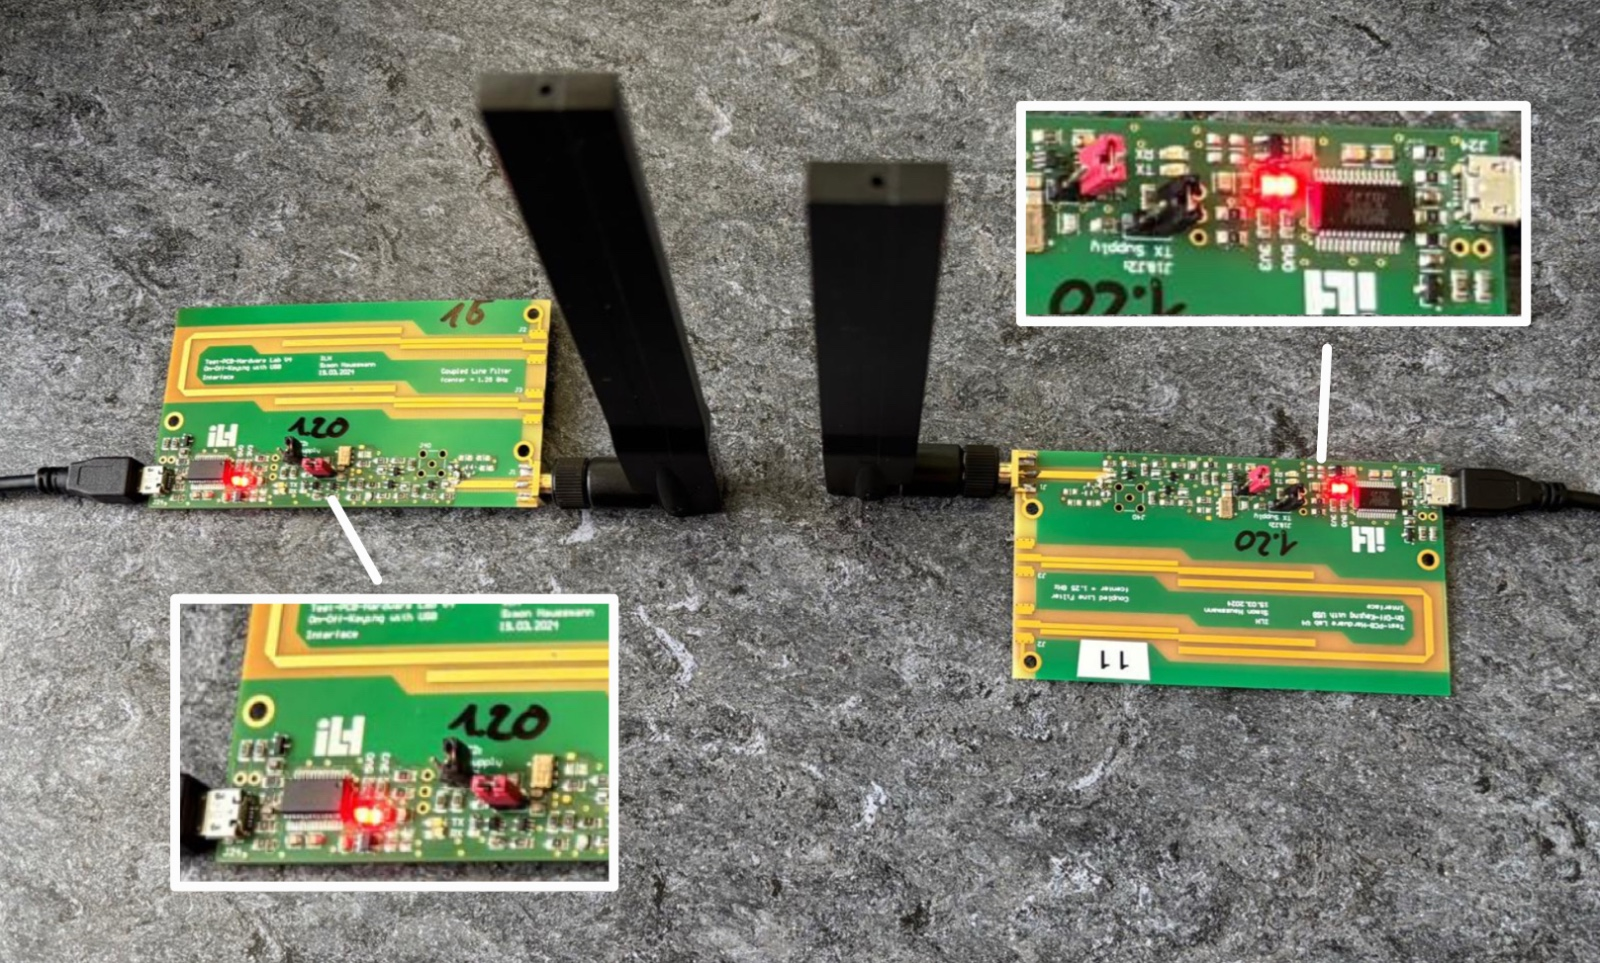
\includegraphics[width=0.8\textwidth]{Pictures/Task2aa.jpg}
    \caption{Sender und Empfänger innerhalb der Funkreichweite}
    \label{fig:Task2aa}
\end{figure}

\begin{figure}[H]
    \centering
    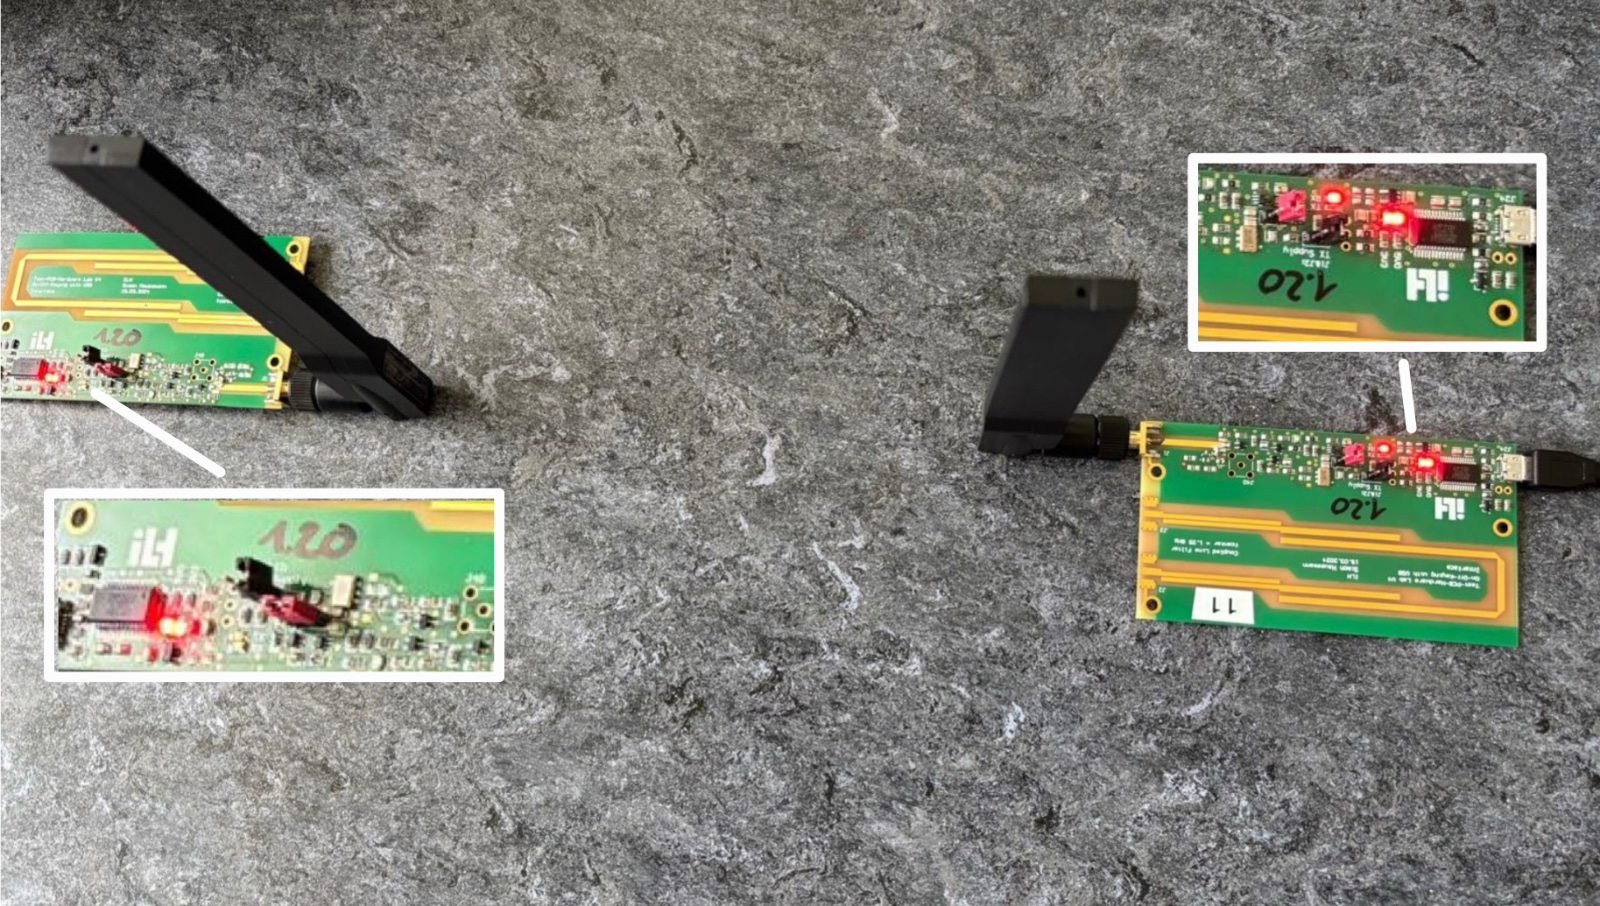
\includegraphics[width=0.8\textwidth]{Pictures/Task2a.jpg}
    \caption{Sender und Empfänger außerhalb der Funkreichweite}
    \label{fig:Task2a}
\end{figure}
Nun betrachten wir die Funkreichweite der Platinen genauer. Diese Messung führen wir auf zwei unterschiedliche
Arten durch. Einmal wird der Abstand der beiden Antennen innerhalb der Funkreichweiter erhöht bis der Kontakt
abbricht. Dann wird der Abstand der Antennen außerhalb der Funkreichweite verringert bis der Kontakt wieder
hergestellt ist. Zuerst wurd eine Funkreichweite von $d_{TR,1}=9cm$ gemessen. Auf die zweite Art wurde eine
Funkreichweite von $d_{TR,2}=8cm$ gemessen. Dies kann auf das Schwellverhalten des Empfängers (Hysterese-Effekt)
zurückzuführen sein (Evtl. erwähnung in Grundlagen). 
Ein schwaches Signal kann noch von der Platine B empfangen werden, wobei die Verbindung zu unzureichend ist um 
initial erkannt zu werden.\\
Die maximale Funkreichweite der Platinen um Signale sicher auszuwerten beträgt somit $d_{TR,max}=8cm$.
\\
Nun wird der Versuch wiederholt, jeodoch wird die Funktion der Platinen getauscht. Wie zu erwarten ist das Ergbenis
im Rahmen der Messungenauigkeit identisch. Die Funkreichweite beträgt enfalls $d_{TR,1}=9cm$ und $d_{TR,2}=8cm$ und 
hat somit ebenfalls eine maximale Funkreichweite der Platinen um sicher Signale auszuwerten von $d_{TR,max}=8cm$.
\section{Platinen am Computer anschließen}
Nun wurde eine Platine an den Computer angeschlossen und die andere Platine an den Laptop.
Mithilfe von Hterm werden Daten in Form von ASCII-Zeichen von der einen Platine an die andere gesendet
und mit Hterm wieder ausgelesen.
Wichtig in dieser Prozedur war das Verbinden beider Jumper an der Sender-Platine und das Entfernen beider
Jumper an der Empfänger-Platine. 
Wären die Jumper bei der Empfänger-Platine verbunden gewesen, wäre das Problem gewesen, dass die Platine auch 
ein Signal gesendet hätte und dieses auch wieder empfangen hätte, was unerwünscht ist.
In der Praxis konnten wir mit diesem Setup eine nutzbare Reichweite von etwa 7,5 cm erreichen.

\section{Interessante/Witzige Beobachtung}
Als wir die Messung von Task4 durchgeführt haben und dann bei größeren Entfernungen kein Signal mehr erfasst hatten,
haben wir aus Spaß einen Samsung-Pen auf beide Antennen gelegt und aufeinmal konnten wir wieder Signale empfangen.
Ein möglicher Grund dafür könnte sein, dass der Samsung-Pen metallische Bestandteile enthält,
die die EM-Welle besser leiten als Luft.

\begin{figure}[H]
    \centering
    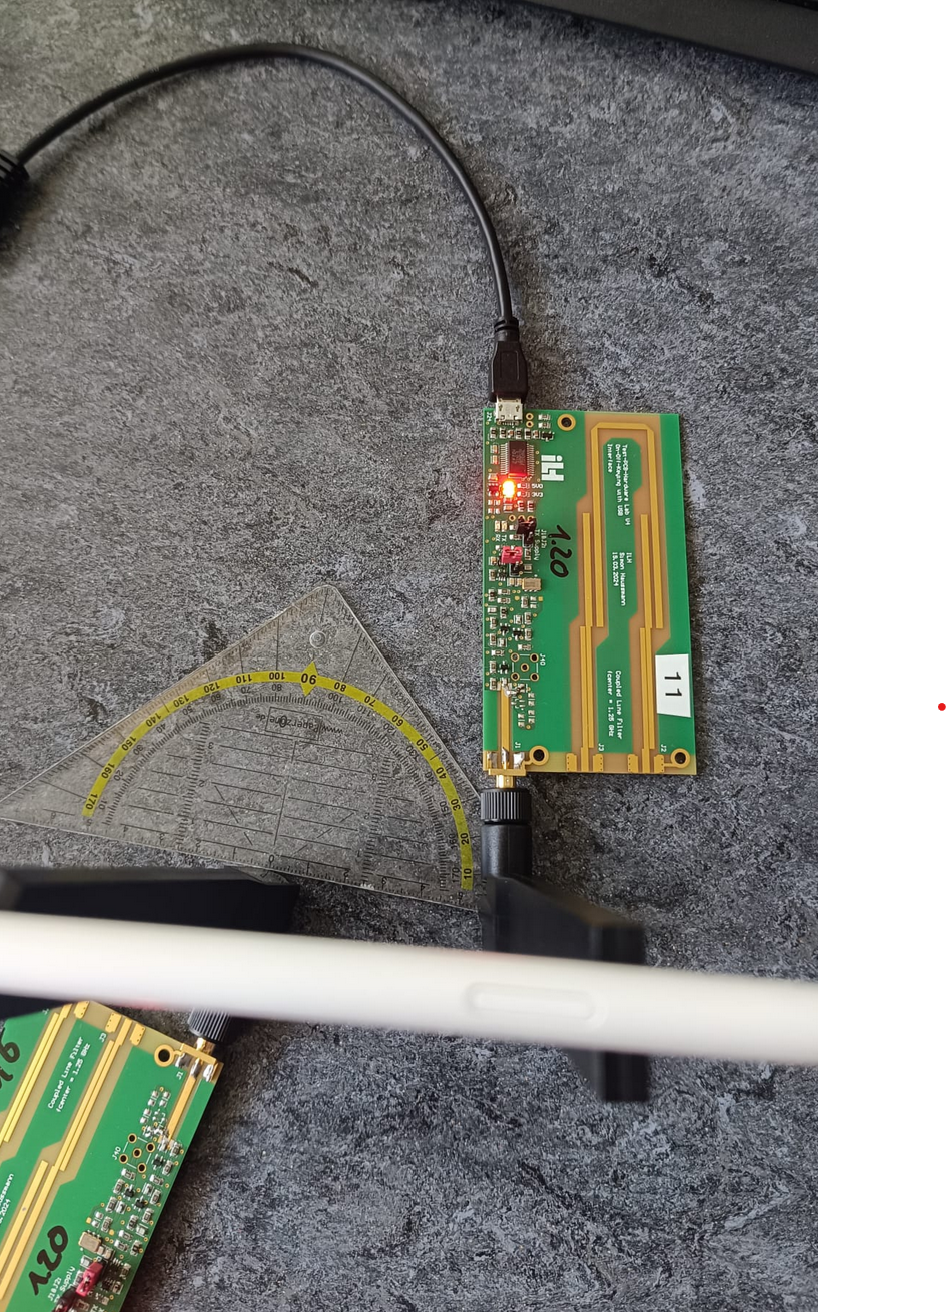
\includegraphics[width=0.4\textwidth]{Pictures/stift.png}
    \caption{Samsung Pen auf Antenne}
\end{figure}



\section{Bildübertragung über Funkverbindung}
Zu guter Letzt wird eine Bildübertragung eine sehr kurze Funkstrecke durchgeführt. Das folgende Originalbild wird hierbei übertragen:
\begin{figure}[H]
    \centering
    
\includegraphics[width=0.6\textwidth]{Pictures/meme.jpg}
    \caption{Das zu übertragende Originalbild}
    \label{fig:Task2b}
\end{figure}

Das Bild wird als eine Ansammlung von ASCII-Zeichen übertragen, da eine Übertragung als Bild im Originalformat (.png) aus technischen Gründen nicht möglich ist.
Ein eher verbreiteter Format der binären Bilderübertragung ist das Base64-Format. Jedoch kann dieses nicht hier verwendet werden, das es nicht zur Verfügung steht.

\subsection{Übertragung bei sehr kurzer Funkstrecke}
Ein Ausschnitt aus der Sammlung der ASCII-Zeichen, die übertragen wurde, ist in Abbildung \ref{fig:Task2c} zu sehen.

\begin{figure}[H]
    \centering
    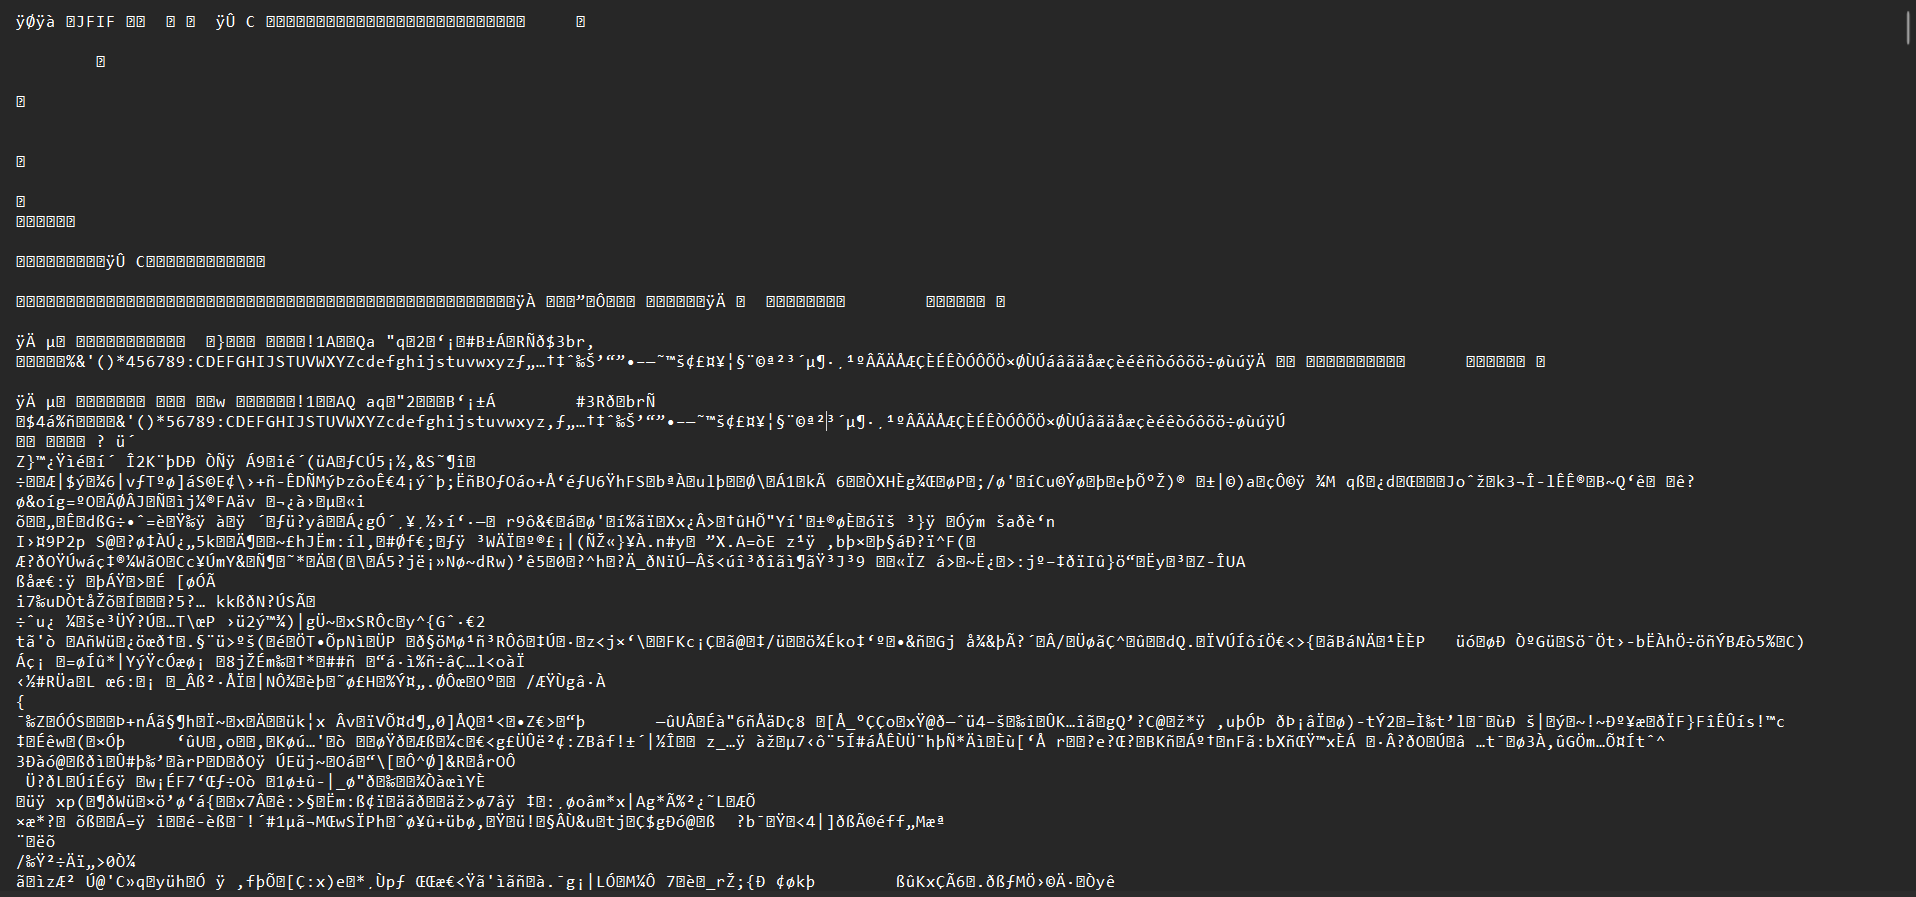
\includegraphics[width=0.8\textwidth]{Pictures/memeASCII.png}
    \caption{Das übertragene Bild in ASCII-Darstellung}
    \label{fig:Task2c}
\end{figure}

In dem Format ist die Datei für den Menschen nicht lesbar, da sie aus einer Vielzahl von Zeichen besteht, die nicht direkt interpretiert werden können. 
Die Änderung der Dateierweiterung in .png stellt sicher, dass das Bild tatsächlich als ein Bild dargestellt wird. 

Die Datei lässt sich hierbei bei einer sehr kurzen Funkstrecke problemlos öffnen, was davon überzeugt, dass die Fehlerbitrate bei einer geringen bzw. gar nicht vohandenden Distanz zwischen Sender und Empfänger sehr gering ist.

\subsection{Übertragung bei größerer Funkstrecke}
Wird jetzt aber einge längere Funkstrecke zwischen Sender und Empfänger gewählt, so ändert sich das Verhalten der Übertragung. 

Es stellte sich in der Praxis heraus, dass die Übertragungsqualität bei einer größeren Funkstrecke deutlich abnimmt, nämlich quadratisch mit der Entfernung.

In der Abbildung \ref{fig:Task2d} sind die Bilder zu sehen, die mit kleiner werdender Funkstrecke übertragen wurden.
\begin{figure}[H]
    \begin{minipage}{0.45\textwidth}
            \centering
            
\includegraphics[width=\linewidth]{Pictures/grosserAbstand.jpg}
        \end{minipage}
        \hfill
        \begin{minipage}{0.45\textwidth}
            \centering
            
\includegraphics[width=\linewidth]{Pictures/wenigergrosserabstand.jpg}
        \end{minipage}

        \vspace{0.5cm}

        \begin{minipage}{0.45\textwidth}
            \centering
            
\includegraphics[width=\linewidth]{Pictures/nochwenigergrosserabstand.jpg}
        \end{minipage}
        \hfill
        \begin{minipage}{0.45\textwidth}
            \centering
            
\includegraphics[width=\linewidth]{Pictures/kleinerabstand.jpg}  
        \end{minipage}   
    \caption{Das übertragene Bild bei verschiendenen Funkstrecken}
    \label{fig:Task2d} 
    \end{figure}


Man sieht deutlich, dass die Übertragung bei größerer Funkstrecke zu Störungen führt, die sich in Form von fehlenden Pixeln im Bild äußern. 
In der Praxis war die Änderung des Abstands im Bild 4 relativ zu Bild 3 vegleichsweise klein, hatte jedoch eine massive Verbesserung der Übertragungsqualität zur Folge, 
welche sich mathematisch durch den Gewinn $G$ ausdrücken lässt: 
\begin{equation}
    G = \frac{P_\text{TX}}{P_\text{RX}}
\end{equation}
wobei $P_\text{TX}$ die von der Antenne auf der Senderseite abgestrahlte Leistung und $P_\text{RX}$ die der Antenne auf der Empfängerseite zugeführte Leistung ist.
\clearpage
Bewegt man die Platinen während der Übertragung, so kann es zu Störungen kommen, die die Übertragung beeinträchtigen. Das Ergebnis der Bildübertragung ist dann das folgende:
\begin{figure}[H]
    \centering
    
\includegraphics[width=0.6\textwidth]{Pictures/memeASCIIbewegt.jpg}
    \caption{Das übertragene Bild in ASCII bei bewegten Platinen}
    \label{fig:Task2e}
\end{figure}
Bei der oberen Darstellung ist zu beachten, dass aufgrund der LaTeX-Formatierung das Bild im unteren Teil, das nicht korrekt übertragen wurde, schwarz gefärbt ist. Der untere Teil müsste aber weiß sein, da dies die automatische Hintergrundfarbe von inkorrekt übertragenen Zeichen ist. 